\documentclass{book}

\usepackage{../Package/latexa}
\usepackage{../Package/algebra}
\usepackage{../Package/theorema}
\usepackage{../Package/diagramma}
\usepackage{../Package/categoria}

\usepackage{tikz}
\usepackage{tikz-cd}
\usetikzlibrary{arrows}

\newcommand{\qi}{\backsimeq_{\textsc{QI}}}
\newcommand{\ba}{\backsimeq_{\textsc{BA}}}
\newcommand{\normal}{\vartriangleleft}
\newcommand{\tm}{\subset}
\newcommand{\Stab}[2]{\textsf{Stab}_{#1}(#2)}
\newcommand{\Cay}[2]{\textsf{Cay}(#1,#2)}

\renewcommand{\C}{\mathcal{C}}
\newcommand{\Cz}{\mathbb{C}}

\renewcommand{\i}{^{-1}}

\newcommand{\pf}{\mathfrak{p}}

\begin{document}

\tableofcontents

\chapter{Topologische Gruppen}
\section{Topologische Gruppen}
\Def{Topologische Gruppen}
Ein Paar $(G,\T)$ einer Gruppe und einer Topologie auf $G$ heißt \df{topologische Gruppe}, wenn die Abbildungen
\begin{align*}
\_\cdot\_ : G \times G &\Pfeil{} G\\
\_\i : G &\Pfeil{} G
\end{align*}
stetig sind.\\
Unter einem \df{Homomorphismus topologischer Gruppen} verstehen wir einen stetigen Gruppenhomomorphismus.

\Bem{}
Seien $G,H$ topologische Gruppen.
\begin{itemize}
\item $U \subset G$ heißt \df{Umgebung} von $g\in G$, falls eine Teilmenge $V \subset_o G$ existiert, sodass $g \in V \subseteq U$.
\item $\phi: G \pfeil{} H$ ist genau ein Homomorphismus, wenn das Urbild jeder Umgebung der 1 in $H$ eine Umgebung der 1 in $G$ ist.
\end{itemize}

\Prop{}
\label{Prop4}
Sei $G$ eine topologische Gruppe und $U \subset G$ eine Umgebung der 1.
\begin{itemize}
\item[(i)] Es existiert eine offene Umgebung $V$ der 1, sodass $V\cdot V \subset U$ und $V = V\i$.
\item[(ii)] Es existiert eine Umgebung $V$ der 1, deren Abschluss $\overline{V}$ in $U$ enthalten ist.
\end{itemize}
Sei nun $H \leq G$ eine Untergruppe.
\begin{itemize}
\item[(iii)] Der Abschluss von $H$ ist ebenfalls eine Untergruppe. Dieser ist insbesondere normal, falls $H$ ebenfalls normal ist.
\item[(iv)] Ist $H \leq_o G$ offen, so auch abgeschlossen, also insbesondere eine Zusammenhangkomponente.
\end{itemize}
\begin{Beweis}{}
\begin{itemize}
\item[(i)] Definiere
\begin{align*}
f&: G \pfeil{} G, x \mapsto x^2\\
V' &:= f\i(U) \cap U\\
V &:= V' \cap {V'}\i
\end{align*}
\item[(ii)] Wir geben ohne Beweis einen Satz an, aus dem die Behauptung sofort folgt:
\paragraph{Satz von Weil}
Eine topologische Gruppe $G$ ist $\text{T}_{3\frac{1}{2}}$, d.\,h., ist $A\subseteq_aG$ eine Teilmenge, die die 1 nicht enthält, so existiert eine stetige Abbildung $f : G \pfeil{} [0,1] \subset \R$ mit folgenden Eigenschaften:
\begin{itemize}
\item $f(A) = \{1\}$
\item $f(1) = 0$
\end{itemize}
\item[(iii)] Seien $a,b \in \overline{H}$, dann existieren Folgen $a_n,b_n \in H$, die gegen $a,b$ konvergieren. Dann ist $(a_n,b_n\i)$ eine Folge in $G\times G$, die gegen $(a,b\i)$ konvergiert. Da Multiplikation stetig ist, konvergiert $a_nb_n\i \in H$ gegen $ab\i$, ergo liegt $ab\i$ in $\overline{H}$. Analog zeigt man, dass $\overline{H}$ normal ist, falls $H$ normal ist.
\item[(iv)] Sei $H \leq_o G$ offen und sei $a \in \overline{H}$. Dann existiert eine Folge $a_n \in H$, die gegen $a$ konvergiert. $aH$ ist eine Umgebung von $a$, ergo existiert ein $N \in \N$, sodass $a_n \in aH$. Daraus folgt $a \in a_nH\i = H$.
\end{itemize}
\end{Beweis}

\Prop{}
\label{Prop5}
Sei $G$ eine topologische Gruppe. Dann sind folgende Aussagen äquivalent:
\begin{itemize}
\item[(i)] $G$ ist hausdorffsch.
\item[(ii)] $\{1\}$ ist abgeschlossen in $G$.
\item[(iii)] $\{g\}$ ist abgeschlossen in $G$ für alle $g \in G$.
\end{itemize}
\begin{Beweis}{}
Es bleibt die Implikation (iii) $\Impl{}$ (i) zu zeigen. Seien $g,h \in G$ verschieden. Dann ist $U = G \setminus \{gh\i\}$ offen in $G$. Laut Proposition \ref{Prop4} (i) existiert eine offene Teilmenge $V$ von $U$ mit folgenden Eigenschaften:
\begin{itemize}
\item $1\in V$
\item $VV \subset U$
\item $V\i = V$
\end{itemize}
Dann sind $Vg, Vh$ disjunkte Umgebungen von $g,h$. Denn wäre ihr Schnitt nichtleer, so würden $v,w\in V$ existieren, sodass $vg  = wh$, woraus folgt dass $gh\i $ in $ U$ liegen würde.
\end{Beweis}

\Prop{}
\label{Prop6}
Sei $G$ eine topologische Gruppe und $H \leq G$ eine Untergruppe.
\begin{itemize}
\item[(i)] $H$ ist genau dann diskret, wenn $H$ einen isolierten Punkt besitzt.
\item[(ii)] Ist $G$ hausdorffsch und $H$ diskret, so ist $H$ abgeschlossen.
\end{itemize}
\begin{Beweis}{(ii)}
$H$ ist diskret, d.\,h., es existiert eine offene Teilmenge $V \subseteq_o G$, s.\,d. $V \cap H = \{1\}$. Ohne Einschränkung darf angenommen werden, dass $V = V\i$.\\
G ist hausdorffsch, ergo ist $\{1\}$ abgeschlossen in $V$. Sei $x \in \overline{H}$, dann existiert ein $y \in H$, das in $xV$ liegt. Man erhält durch Umformung
\[ x \in yV \cap \overline{H} = \bigcap_{H \subset A \subset_a G} A \cap yV = \bigcap_{\{y\} = H \cap yV \subset A \subset_a yV} A  = \{y\} \]
Ergo gilt $x = y \in H$.
\end{Beweis}

\Prop{}
\label{Prop1.1.8}
Sei $G$ eine topologische Gruppe mit Untergruppe $H$.
\begin{itemize}
\item $G$ operiert stetig auf $G/H$.
\item $\pi_H : G \pfeil{} G/H$ ist eine offene Abbildung.
\item $G/H$ ist genau dann hausdorffsch, wenn $H$ abgeschlossen ist.
\item $G/H$ ist genau dann diskret, wenn $H$ offen ist.
\item Ist $H$ normal, so ist $G/H$ eine topologische Gruppe und $\pi_H$ ein Morphismus topologischer Gruppen.
\end{itemize}
\begin{Beweis}{(iii)}
 $\Longrightarrow$: Sei $a \in \overline{H}$, dann existiert eine Folge $a_n \in H$, die gegen $a$ konvergiert. Da $\pi_H$ stetig ist, gilt
\[ \pi_H(a_n) \Pfeil{n\pfeil{} \infty} \pi_H(a) \]
Da alle $a_n$ in $H$ liegen, gilt aber $\pi_H(a_n) = \pi_H(1)$. Da $G/H$ hausdorffsch ist, besitzt diese Folge höchstens einen Grenzwert, ergo gilt
\[ \pi_H(a) = \pi_H(1) \Impl{} a \in H \]
$\Longleftarrow$: Seien $\pi_H(b),\pi_H(c) \in G/H$. Ohne Einschränkung nehmen wir an, dass $\pi_H(c) = \pi_H(1)$.\\
In jeder Umgebung $\widetilde{U}$ von $\pi_H(b)$ sei $\pi_H(1)$ enthalten. Dann ist $b$ im Abschluss von $H$ enthalten, denn ist $U$ eine Umgebung von $b$, so ist $\pi(U)_H$ eine Umgebung von $\pi_H(b)$. Ergo ist $\pi_H(1) \in \pi_H(U)$, ergo existiert ein $h \in H$, sodass $h \in U$.
\end{Beweis}

\Def{}
Ist $G$ eine topologische, so ist $\overline{\{1\}}$ normal. $G/\overline{\{1\}}$ wird als \df{Hausdorffquotient} von $G$ bezeichnet.

\Def{}
Ein Homomorphismus $\phi : G \pfeil{} G'$ topologischer Gruppen heißt \df{strikt}, falls er den Isomorphiesatz respektiert, d.\,h., die induzierte Abbildung
\[ \phi : G / \Ker \phi \Pfeil{} \Img \phi \]
ist homöomorph.

\Def{}
Eine kurze exakte Sequenz topologischer Gruppen heißt \df{topologisch exakt}, falls alle beteiligten Abbildungen strikt sind.

\section{Lokal-Kompakte Gruppen}
\Def{}
Sei $X$ ein topologischer Raum.
\begin{itemize}
\item Wir nennen $X$ \df{kompakt}, falls er \df{quasikompakt} ist, d.\,h., jede offene Überdeckung von $X$ besitzt eine offene Teilüberdeckung.
\item $X$ heißt \df{lokal kompakt}, falls jeder Punkt eine Umgebung enthält, deren Abschluss kompakt ist.
\end{itemize}

\Bem{}
\begin{itemize}
\item Jede abgeschlossene Teilmenge eines kompakten Raumes ist kompakt.
\item Jede kompakte Menge eines Hausdorffraums ist abgeschlossen.
\item Ist ein Raum kompakt und hausdorffsch, so erfüllt er \df{T3}, d.\,h., er ist \df{regulär}, d.\,h., jede abgeschlossene Teilmenge und jeder nicht in dieser Teilmenge liegender Punkt könne durch offene Umgebungen getrennt werden.
\item Ein Raum ist genau dann regulär, wenn jeder Punkt eine Umgebungsbasis aus abgeschlossenen Umgebungen besitzt.
\item In lokal kompakten Räumen hat jeder Punkt eine Umgebungsbasis aus kompakten Umgebungen.
\item Ist ein Raum kompakt und hausdorffsch, so erfüllt er \df{T4}, d.\,h., er ist \df{normal}, d.\,h., disjunkte abgeschlossene Teilmengen werden durch offene Umgebungen getrennt.
\item Eine bijektive, stetige Abbildung von einem Kompaktum nach einem Hausdorffraum ist homöomorph.
\end{itemize}

\Prop{}
Sei $G$ eine lokal kompakte Gruppe, $H\leq G$ eine abgeschlossene Gruppe.
\begin{itemize}
\item $G/H$ ist ein lokal kompakter Raum.
\item Jede kompakte Teilmenge von $G/H$ besitzt ein kompaktes Urbild.
\end{itemize}

\Prop{}
Sei $G$ lokal kompakt und hausdorffsch, $H \leq G$ eine Untergruppe.\\
$H$ ist genau dann diskret, wenn $H\cap K$ für alle kompakten Teilmengen von $K \subset G$ endlich ist.

\section{Zusammenhangkomponenten}
\Def{}
Ein topologischer Raum heißt \df{zusammenhängend}, wenn er sich nicht in zwei offene, disjunkte, nichtleere Teilräume zerlegen lässt.

\Bem{}
\begin{itemize}
\item Ist eine Teilmenge eines Raumes zusammenhängend, so ist es auch ihr Abschluss.
\item Seien $A_i \subset X$ jeweils zusammenhängend, dann gilt
\[ \bigcap_{i\in I}A_i \neq \emptyset \Impl{} \bigcup_{i\in I} A_i \text{ ist zusammenhängend} \]
\item Beliebige Produkte zusammenhängender Räume sind zusammenhängend.
\item Bilder zusammenhängender Räume bleiben unter stetigen Abbildungen zusammenhängend.
\end{itemize}

\Def{}
Sei $X$ ein topologischer Raum.
\begin{itemize}
\item Ist $x \in X$ ein Punkt, so verstehen wir unter der \df{Zusammenhangkomponente} von $x$ die größte, zusammenhängende Teilmenge von $X$, die $x$ enthält.
\item $X$ heißt \df{total unzusammenhängend}, wenn jede Zusammenhangkomponente genau ein Element enthält.
\item Ist $G$ eine topologische Gruppe, so bezeichnen wir mit $G^o$ die Zusammenhangkomponente der Eins. 
\end{itemize}

\Prop{}
Ist $G$ eine topologische Gruppe, so ist $G^o$ ein abgeschlossener Normalteiler.

\Prop{}
Sei $G$ eine topologische Gruppe, $H \leq G$ eine Untergruppe. Sind $H$ und $G/H$ zusammenhängend, so auch $G$.

\Prop{}
Sei $G$ eine topologische Gruppe, dann ist $G/G^o$ hausdorffsch und total unzusammenhängend.

\Bem{}
Eine total unzusammenhängende Gruppe ist hausdorffsch.

\section{Total Unzusammenhängende Gruppen}
\Satz{}
Eine hausdorffsche Gruppe ist genau dann total unzusammenhängend und lokal kompakt, wenn jede Umgebung der Eins eine offene und kompakte Untergruppe enthält.

\Lem{}
Sei $X$ ein kompakter und total unzusammenhängender Hausdorffraum. Bezeichnet $\mathcal{W}$ für $x \in X$ die Menge der Umgebungen von $x$, die zugleich offen und abgeschlossen sind, so gilt
\[ \bigcap_{W\in \mathcal{W}} W = \{x\} \]

\Lem{}
Sei $G$ eine lokal kompakte und total unzusammenhängende Gruppe, $U$ eine offene Umgebung von $x \in G$.\\
Dann existiert eine offene und kompakte Umgebung von $x$, die in $U$ enthalten ist.

\Kor{}
Sei $G$ eine kompakte und total unzusammenhängende Gruppe. Dann enthält jede Umgebung der Eins einen offenen Normalteiler.

\section{Limiten Topologischer Räume}
\Def{Gerichtet Geordnet}
Sei $I$ eine nichtleere Menge.
\begin{itemize}
	\item $(I,\leq)$ heißt \df{teilgeordnet}, falls $\leq$ auf $I$ eine binäre Relation ist, die reflexiv und transitiv ist.
	\item Eine teilgeordnete Menge $(I,\leq)$ heißt \df{gerichtet}, falls für jedes Paar $i,j \in I$ ein $k \in I$ existiert, sodass $i \leq k$ und $j\leq k$.
\end{itemize}

\Def{Inverses System}
Sei $I$ gerichtet.
\begin{itemize}
	\item Ein \df{inverses System} $(X_i, \phi_{ij})$ topologischer Räume ist ein kontravarianter Funktor $X : I \pfeil{} \Top$, d.\,h., die $X_i$ sind topologische Räume und für jedes $i\leq j$ ist
	\[\phi_{ij} :X_j \Pfeil{}X_i \]
	eine stetige Abbildung.
	\item Ein Morphismus inverser Systeme ist eine natürliche Transformation von inversen Systemen.
	\item Ist $X$ ein topologische Raum, so verstehen wir unter $(X, \id{X})$ das \df{konstante System} zu $X$.
\end{itemize}

\Def{Projektiver Limes}
Ein \df{projektiver bzw. inverser Limes} eines inversen Systemes $(X_i, \phi_{ij})$ ist ein topologischer Raum
\[ X = \lim\limits_{i \in I}(X_i, \phi_{ij}) =: \lim\limits_{i\in I}X_i \]
der den Funktor
\begin{align*}
\Top &\Pfeil{} \textbf{Set}\\
Y & \longmapsto \Hom{\text{inv.Sys.}}{(Y,\id{Y})}{(X_i, \phi_{ij})}
\end{align*}
darstellt, d.\,h.,
\[ \Hom{\Top}{Y}{X}  \isom{} \Hom{\text{inv.Sys.}}{(Y,\id{Y})}{(X_i, \phi_{ij})} \]

\Bem{}
\begin{itemize}
	\item Ein Limes ist eindeutig bis auf eindeutige Isomorphie.
	\item Folgendes Konstrukt ist ein Limes von $(X_i, \phi_{ij})$
	\[ X:= \set{(x_k) \in \prod_{i\in I}X_i }{ \phi_{ij}(x_i) = x_j \forall i \leq j } \]
	\item Es gilt
	\[ X= \bigcap_{i\leq j} \set{(x_k) \in \prod_{i\in I}X_i }{ \phi_{ij}(x_i) = x_j} \]
\end{itemize}

\Prop{}
Sei $(X_i, \phi_{ij})$ ein inverses System topologischer Räume mit stetigen Abbildungen
\[ \phi_i : X_i \Pfeil{} X:= \lim\limits_{i \in I} X_i \]
\begin{itemize}
	\item Die $\phi_i\i$ bilden für alle $i$ und $U\subseteq_o X_i$ eine Basis der Topologie von $X$.
	\item Eine Teilmenge $Y \subset X$ mit $\phi_i(Y) = X_i$ für alle $i\in I$ liegt dicht in $X$.
	\item Eine Abbildung $f : X \pfeil{} Y$ ist genau dann stetig, wenn für alle $i \in I$ $\phi_i\circ f$ stetig ist.
\end{itemize}
\Prop{}
Sei $(X_i,\phi_{ij})$ ein inverses System topologischer Räume mit Limes $X$.
\begin{itemize}
	\item Sind alle $X_i$ hausdorffsch, so ist dies auch $X$.
	\item Sind alle $X_i$ total unzusammenhängend, so auch $X$.
	\item Sind alle $X_i$ hausdorffsch, so ist
	\[\set{(x_k) \in \prod_{i\in I}X_i }{ \phi_{ij}(x_i) = x_j \forall i \leq j }\]
	eine abgeschlossene Teilmenge von $\prod_{i \in I}X_i$.
	\item Sind alle $X_i$ kompakt und hausdorffsch, so ist es auch $X$.
	\item Sind alle $X_i$ nichtleer, kompakt und hausdorffsch, so ist dies auch $X$.
\end{itemize}
\Prop{}
Seien folgende Morphismen inverser Systeme von kompakten und hausdorffschen Gruppen gegeben
\begin{align*}
 (F_i, \upsilon_{ij}) \Pfeil{\alpha} (G_i, \phi_{ij}) \Pfeil{\beta} (H_i, \chi_{ij})
\end{align*}
Ist diese Sequenz gradweise exakt, d.\,h., ist für alle $i \in I$
\[ F_i \Pfeil{\alpha_i} G_i \Pfeil{\beta_i} H_i \]
exakt, so ist auch die Limessequenz
\[ \lim\limits_{i\in I} F_i \Pfeil{\alpha} \lim\limits_{i \in I}G_i \Pfeil{\beta} \lim\limits_{i \in I}H_i \]
exakt.

\Def{Kolimes}
Sei $I$ gerichtet.
\begin{itemize}
	\item Ein \df{direktes System} topologischer Räume ist ein kovarianter Funktor
	\[X : I \Pfeil{} \Top\]
	\item Morphismen direkter System sind natürliche Transformationen der zugrunde liegenden Funktoren.
	\item Ein \df{Kolimes} eines direkten Systemes $(X_i, \phi_{ij})$ ist ein topologischer Raum $X = \textsf{colim}_{i\in I}X_i$, der den Funktor
	\[ Y \longmapsto \Hom{}{(X_i,\phi_{ij})}{(Y,\id{Y})} \]
	darstellt.
\end{itemize}

\Bem{}
Ist $(X_i,\phi_{ij})$ ein direktes System, so ist folgender Kolimes gegeben
\[ \coprod_{i\in I}X_i/\sim \]
wobei
\[ x_i \sim x_j \Gdw{} \exists k \geq i,j : \phi_{ik}(x_i) = \phi_{jk}(x_j) \]

\section{Proendliche Gruppe}
\Bem{}
Jede endliche Gruppe wird als eine topologische Gruppe aufgefasst, indem wir sie mit der diskreten Topologie versehen.
\Def{}
Eine topologische Gruppe heißt \df{proendlich}, wenn sie ein projektiver Limes eines inversen Systems endlicher Gruppen ist.
\Satz{}
Sei $G$ eine topologische Gruppe. Folgende Aussagen sind äquivalent:
\begin{itemize}
	\item $G$ ist proendlich.
	\item $G$ ist kompakt und total unzusammenhängend.
	\item $G$ ist kompakt und
	\[ \bigcap_{N\trianglelefteq_o G}N = \{1\} \]
\end{itemize}

\Lem{}
Sei $G$ eine topologische Gruppe, $I$ eine Familie abgeschlossener Normalteiler, sodass gilt
\[ N_1,N_2 \in I \Impl{} \exists N_3 \in I: N_3 \subseteq N_1 \cap N_2 \]
\begin{itemize}
	\item Definiere für $N_1,N_2\in I$
	\[ N_1\preceq N_2 \Gdw{} N_1 \supseteq N_2 \]
	Dann ist $(I,\preceq)$ gerichtet.
	\item Setzt man für $N_i \preceq N_j$
	\[ \phi_{ij} : G/N_j \Pfeil{} G/N_i \]
	so ist $(G/N_i, \phi_{ij})$ ein inverses System.\\
	Definiere
	\[ \widehat{G} := \lim\limits_{N \in I}G/N \]
	Es existiert ein kanonischer Morphismus stetiger Gruppen
	\[ \upsilon : G \Pfeil{} \widehat{G} \]
	mit Kern
	\[\Ker \upsilon = \bigcap_{N\in I}N \]
	\item Ist $G$ kompakt, so ist $\upsilon$ surjektiv.
\end{itemize}

\section{Unendliche Galoistheorie}

\Satz{}
Sei $L|K$ eine galoissche, nicht notwendigerweise endliche Körpererweiterung. Definiere
\[ G(L|K) :=\Aut{K-\text{Alg.}}{L} \]
$G(L|K)$ erhält eine Topologie als Gruppe, indem wir Untergruppen der Gestalt
\[ G(L|E) \]
für alle endlichen, galoisschen Teilerweiterungen $E|K$ zu einer Umgebungsbasis der Eins in $G(L|K)$ zusammenfassen. Es gilt dann
\[ G = \lim\limits_{\stackrel{L|E|K}{E|K \text{ endl., gal.}}}G(E|K) \]

\Satz{Satz der Unendlichen Galoistheorie}
Für eine galoissche Körpererweiterung  $K$ herrschen folgende Dualitäten vor
\begin{center}
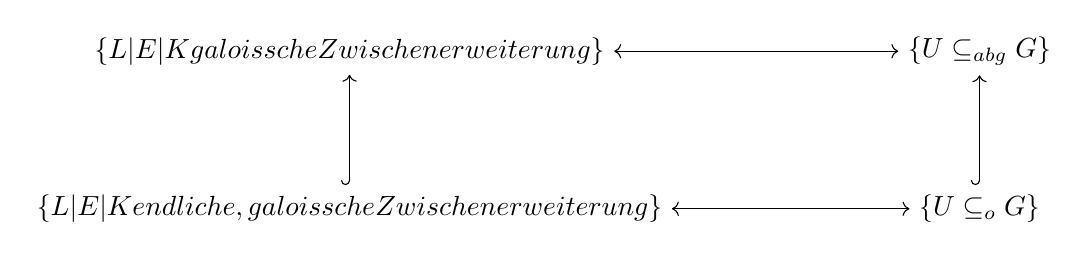
\begin{tikzpicture}[scale =2]
\node (D1) at (0,1)  {$\{L|E|K\text{ galoissche Zwischenerweiterung}\}$};
\node (D3) at (4,1)  {$\{ U \subseteq_\text{abg} G \}$};
\node (D5) at (4,0)  {$\{U \subseteq_o G \}$};
\node (D7) at (0,0)  {$\{L|E|K\text{endliche, galoissche Zwischenerweiterung}\}$};

\draw[<->] (D1) -> (D3);
\draw[<->] (D5) -> (D7);
\draw[right hook->] (D5) -> (D3);
\draw[right hook->] (D7) -> (D1);
%\draw [ultra thick, right hook->,    blue] (0,-1) -- (3,-1);
\end{tikzpicture}
\end{center}
durch
\begin{align*}
E & \longmapsto G(L|E)\\
H & \longmapsto L^H
\end{align*}



\chapter{Klassenkörpertheorie -- Motivation und Hauptresultate}
\section{Abelsche und Quadratische Erweiterungen von $\Q$}
\Satz{Kroncker-Weber}
Sei $L|\Q$ eine endliche Erweiterung. Folgende Aussagen sind äquivalent:
\begin{itemize}
	\item $L|\Q$ ist abelsch.
	\item $L$ ist enthalten in einem Kreisteilungskörper $\Q(\mu_n)$.
\end{itemize}

\Satz{}
Sei $N \in \N$, $L |\Q$ endlich. Folgende Aussagen sind äquivalent:
\begin{itemize}
	\item $L \subseteq \Q(\mu_N)$.
	\item Ob eine Primzahl $p$ in $L$ voll zerlegt ist, hängt nur von $p\mod{n}$ ab.
\end{itemize}

\Satz{}
Sei $L|\Q$ abelsch und $N$ minimal mit
\[ L \subseteq \Q(\mu_N) \]
Für jede Primzahl $p$ gilt
\[ p \text{ ist in }L \text{ verzweigt} \Gdw{} p|N \]

\Satz{}
Sei $N \in \N$ und $H \subseteq (\Z/N\Z)^\times \isom{} G(\Q(\mu_N) / \Q)$ beliebig. Es bezeichne $L = \Q(\mu_N)$.\\
Für $p\not | N$ prim gilt:
\begin{itemize}
	\item $p$ ist unverzweigt in $L$.
	\item $p$ ist genau dann voll zerlegt in $L$, wenn $p\mod{N} \in H$.
	\item Ist $f$ die kleinste natürliche Zahl, die
	\[ p^f \mod{N} \in H \]
	erfüllt, so ist $p\O_L$ ein Produkt von $[L:\Q]/f$ verschiedenen Primidealen. 
\end{itemize}

\Prop{}
Sei $L|K$ galoissch und $\pf \subset \O_K$ unverzweigt in $L$. Dann gilt
\begin{itemize}
	\item 
\end{itemize}

\end{document}